% Rozdział 18 - Grafy 2

\theory{Grafy 2}

\noindent
Rozpatrzmy graf, w którym wierzchołki są podzielone na dwie grupy. Można sobie wyobrazić, że jedna z tych grup to są ,,chłopcy'', a druga ,,dziewczyny''. Przykład takiego grafu z dwoma grupami wierzchołków znajduje się na poniższym rysunku.

\begin{center}
	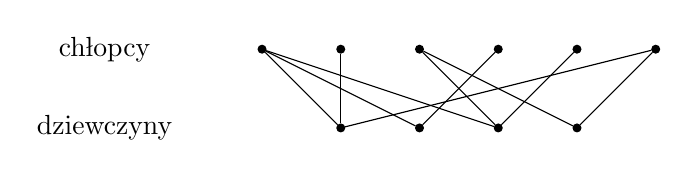
\begin{tikzpicture}
		\tikzset{vertex/.style = {shape=circle,draw, inner sep = 1pt, fill=black}}

		\node (x) at (-2, 0) {dziewczyny};
		\node[vertex] (A_1) at (0,1) {};
		\node[vertex] (A_2) at (1,1) {};
		\node[vertex] (A_3) at (2,1) {};
		\node[vertex] (A_4) at (3,1) {};
		\node[vertex] (A_5) at (4,1) {};
		\node[vertex] (A_6) at (5,1) {};

		\node (x) at (-2, 1) {chłopcy};
		\node[vertex] (B_1) at (1,0) {};
		\node[vertex] (B_2) at (2,0) {};
		\node[vertex] (B_3) at (3,0) {};
		\node[vertex] (B_4) at (4,0) {};




		\draw (A_1)--(B_1);
		\draw (A_6)--(B_4);
		\draw (A_3)--(B_3);
		\draw (A_4)--(B_2);


		\draw (A_1)--(B_2);
		\draw (A_2)--(B_1);
		\draw (A_3)--(B_4);
		\draw (A_1)--(B_3);
		\draw (A_5)--(B_3);
		\draw (A_6)--(B_1);


	\end{tikzpicture}
\end{center}

\noindent
Zastanówmy się, czy w powyższej sytuacji, da się przyporządkować każdej z dziewczyn pewnego chłopaka, tak, aby jeden chłopak był z co najwyżej jedną dziewczyną. Jest to możliwe, co zademonstrowano na poniższym rysunku.

\begin{center}
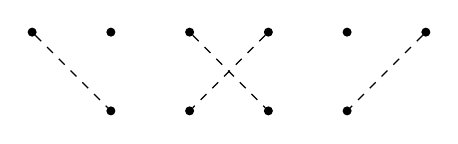
\begin{tikzpicture}
		\tikzset{vertex/.style = {shape=circle,draw, inner sep = 1pt, fill=black}}


		\node[vertex] (A_1) at (0,1) {};
		\node[vertex] (A_2) at (1,1) {};
		\node[vertex] (A_3) at (2,1) {};
		\node[vertex] (A_4) at (3,1) {};
		\node[vertex] (A_5) at (4,1) {};
		\node[vertex] (A_6) at (5,1) {};

		\node[vertex] (B_1) at (1,0) {};
		\node[vertex] (B_2) at (2,0) {};
		\node[vertex] (B_3) at (3,0) {};
		\node[vertex] (B_4) at (4,0) {};




		\draw[dashed] (A_1)--(B_1);
		\draw[dashed] (A_6)--(B_4);
		\draw[dashed] (A_3)--(B_3);
		\draw[dashed] (A_4)--(B_2);



	\end{tikzpicture}
\end{center}



\vspace{10px}
\noindent
Takie przyporządkowanie nazwiemy \textit{skojarzeniem}. Warto zwrócić uwagę, że nie zawsze szukane skojarzenie musi istnieć. W sytuacji zilustrowanej na poniższym rysunku nie da się przyporządkować każdej z dziewczyn innego chłopca.

\begin{center}
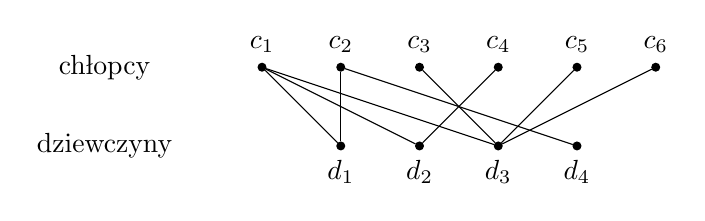
\begin{tikzpicture}
		\tikzset{vertex/.style = {shape=circle,draw, inner sep = 1pt, fill=black}}

		\node (x) at (-2, 0) {dziewczyny};
		\node (x) at (-2, 1) {chłopcy};

		\node[vertex, label=above:$c_1$] (A_1) at (0,1) {};
		\node[vertex, label=above:$c_2$] (A_2) at (1,1) {};
		\node[vertex, label=above:$c_3$] (A_3) at (2,1) {};
		\node[vertex, label=above:$c_4$] (A_4) at (3,1) {};
		\node[vertex, label=above:$c_5$] (A_5) at (4,1) {};
		\node[vertex, label=above:$c_6$] (A_6) at (5,1) {};

		\node[vertex, label=below:$d_1$] (B_1) at (1,0) {};
		\node[vertex, label=below:$d_2$] (B_2) at (2,0) {};
		\node[vertex, label=below:$d_3$] (B_3) at (3,0) {};
		\node[vertex, label=below:$d_4$] (B_4) at (4,0) {};




		\draw (B_1)--(A_1);
		\draw (B_1)--(A_2);
		\draw (B_2)--(A_1);
		\draw (B_3)--(A_1);
		\draw (B_4)--(A_2);
		\draw (B_2)--(A_4);
		\draw (B_3)--(A_5);
		\draw (B_3)--(A_6);
		\draw (B_3)--(A_3);



	\end{tikzpicture}
\end{center}

\vspace{10px}
\noindent
Zauważmy, że dziewczyny $d_1$, $d_3$ i $d_4$ znają jedynie chłopaków $c_1$ i $c_2$. Łatwo wynika stąd, że nie da się każdej z dziewczyn przyporządkować innego chłopaka. Uogólniając tę obserwację mamy
\begin{center}
	jeśli skojarzenie istnieje, to każdy zbiór $k$ dziewczyn zna co najmniej $k$ różnych chłopaków.
\end{center}

\vspace{10px}
\noindent
Czy istnieje taka konfiguracja znajomości, w której dla każdego zbioru dziewczyn zachodzi powyższy warunek, ale skojarzenie nie istnieje? Odpowiedź na powyższe pytanie jest przecząca, o czym mówi twierdzenie Halla o kojarzeniu małżeństw.


\newpage

\heading{Twierdzenie 1 (Halla)}

\noindent
Dana są dwa zbiory -- chłopców i dziewcząt. Niektórzy chłopcy znają się z niektórymi dziewczynami. Wówczas następujące dwa warunki są równoważne:
\begin{enumerate}
	\item istnieje skojarzenie, które każdej dziewczynie przyporządkowuje chłopca;
	\item każdy podzbiór dziewczyn liczący $k$ osób zna co najmniej $k$ chłopców.
\end{enumerate}
% tutaj jakiś rysunek z przykładem o co cho


\heading{Dowód}

\vspace{5px}
\noindent
Wynikanie drugiego warunku z pierwszego jest oczywiste. Wykażemy, że jeśli zachodzi warunek drugi, to musi istniej postulowane skojarzenie.

\vspace{10px}
\noindent
Skorzystamy z indukcji matematycznej po liczbie dziewczyn. Jeśli jest tylko jedna dziewczyna, to teza jest trywialna. Załóżmy, że teza zachodzi dla każdej liczby $d \leqslant n$ dziewczyn -- wykażemy, że jest prawdziwa również dla $n + 1$ dziewczyn.

\vspace{10px}
\noindent
Rozpatrzmy dwa przypadki w zależności od tego, czy istnieje taki podzbiór $k \leqslant n$ dziewczyn, który zna \textit{dokładnie} $k$ chłopców. Załóżmy najpierw, że on istnieje -- nazwijmy go $A$. Zbiór pozostałych dziewczyn nazwijmy $B$. Zbiór chłopaków, którzy są znani przez co najmniej jedną z dziewczyn z $A$ nazwiemy $C_a$, a zbiór pozostałych nazwiemy $C_b$.

\begin{center}
	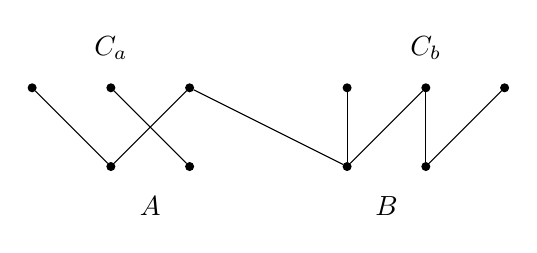
\begin{tikzpicture}
		\tikzset{vertex/.style = {shape=circle,draw, inner sep = 1pt, fill=black}}

		\node[vertex] (A_1) at (0,1) {};
		\node[vertex] (A_2) at (1,1) {};
		\node[vertex] (A_3) at (2,1) {};
		\node (x) at (1, 1.5) {$C_a$};

		\node[vertex] (A_4) at (4,1) {};
		\node[vertex] (A_5) at (5,1) {};
		\node[vertex] (A_6) at (6,1) {};
		\node (x) at (5, 1.5) {$C_b$};

		\node[vertex] (B_1) at (1,0) {};
		\node[vertex] (B_2) at (2,0) {};
		\node (x) at (1.5, -0.5) {$A$};
		\node[vertex] (B_3) at (4,0) {};
		\node[vertex] (B_4) at (5,0) {};
		\node (x) at (4.5, -0.5) {$B$};




		\draw (B_1)--(A_1);
		\draw (B_2)--(A_2);
		\draw (B_1)--(A_3);


		\draw (B_3)--(A_4);
		\draw (B_3)--(A_5);
		\draw (B_4)--(A_5);
		\draw (B_3)--(A_3);
		\draw (B_4)--(A_6);


	\end{tikzpicture}
\end{center}

\vspace{10px}
\noindent
Podzielmy wszystkie osoby na dwa zbiory: $A \cup C_a$ oraz $B \cup C_b$. Wykażemy, że dla każdego z tych zbiorów można zaaplikować założenie indukcyjne. Kojarząc dziewczyny z $A$ z chłopcami z~$C_a$, a dziewczyny z~$B$ z chłopcami z $C_b$ otrzymamy tezę.

\vspace{10px}
\noindent
Żadna dziewczyna z $A$ nie zna nikogo ze zbioru $C_b$. Stąd też warunek $2$ dla zbioru $A \cup C_a$ jest spełniony. Rozpatrzmy dowolny podzbiór $B_1$ zbioru $B$. Wówczas zbiór dziewczyn $A \cup B_1$ zna co najmniej $|A| + |B_1|$ chłopców. Skoro łącznie dziewczyny z $A$ znają dokładnie $|A|$ chłopców, to dziewczyny z $B_1$ muszą łącznie znać ich co najmniej $|B_1|$, czyli warunek~2 jest spełniony.

\vspace{10px}
\noindent
Rozpatrzmy teraz przypadek, w którym każdy zbiór $k \leqslant n$ dziewczyn zna co najmniej $k + 1$ chłopców. Wówczas wybierzmy dowolną dziewczynę. Na mocy założenia zna ona co najmniej jednego chłopaka -- przypiszmy ich sobie. ,,Usuńmy'' ich -- zauważmy, że wówczas warunek 2 będzie spełniony. Istotnie, każdy zbiór $k$ dziewczyn znał $k + 1$ chłopców, więc po usunięciu jednego z nich, znają one ich co najmniej $k + 1 - 1 = k$. Możemy więc na mocy założenia indukcyjnego skojarzyć resztę dziewczyn.

\qed

\newpage

% Source: https://luckytoilet.wordpress.com/2013/12/21/halls-marriage-theorem-explained-intuitively/
\heading{Przykład 1}

\noindent
W pewnym turnieju gra $2m$ drużyn. W ciągu każdego z $2m - 1$ dni każda z drużyn rozgrywała po jednej partii. Każda drużyna zagrała z każdą drużyną dokładnie raz. W żadnym meczu nie było remisów. Wykazać, że można dla każdego dnia wybrać jedną drużynę, która w danym dniu wygrała swój mecz, tak, aby żadna drużyna nie została wybrana więcej niż raz.

\vspace{5px}

\heading{Rozwiązanie}

\vspace{5px}
\noindent
Rozpatrzmy graf, w którym mamy $2m - 1$ wierzchołków, z których każdy odpowiada jednemu z dni, oraz $2m$ wierzchołków, z których każdy odpowiada pewnej drużynie. Wierzchołek odpowiadający drużynie połączymy z wierzchołkiem odpowiadającemu dniowi wtedy i tylko wtedy, gdy dana drużyna wygrała w danym dniu.

\vspace{10px}
\noindent
Chcemy znaleźć skojarzenie przyporządkowujące każdemu dniowi jedną drużynę. Na mocy twierdzenia Halla wystarczy pokazać, że dla dowolnych $k$ dni istnieje co najmniej $k$ drużyn, że każda z nich wygrała podczas jednego z nich. Jeśli każda drużyna wygrała pewien mecz podczas tych $k$ dni, to oczywiście ten warunek jest spełniony. Jeśli istnieje drużyna, która podczas każdego z tych $k$ dni przegrała, to codziennie przegrała z inną drużyną. Toteż jest co najmniej $k$ drużyn, które ją pokonały, czyli w szczególności wygrały co najmniej jeden mecz w rozpatrywanych dniach.

\qed

\vspace{10px}

\heading{Grafy planarne}

\noindent
Grafy, które można narysować na płaszczyźnie tak, aby żadne dwie krawędzie się nie przecinały, nazywamy \textit{grafami planarnymi}. Przykład takiego grafu znajduje się na poniższym rysunku.

\begin{center}
	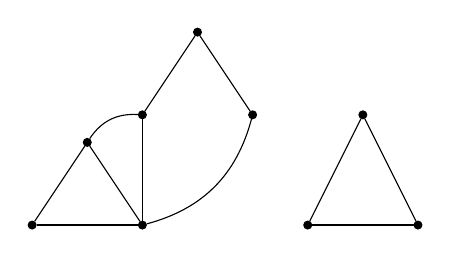
\begin{tikzpicture}[scale=0.7]
		\tikzset{vertex/.style = {shape=circle,draw, inner sep = 1pt, fill=black}}

		\node[vertex] (A_1) at (0,0) {};
		\node[vertex] (A_2) at (1,1.5) {};
		\node[vertex] (A_3) at (2,0) {};
		\node[vertex] (A_4) at (2,2) {};
		\node[vertex] (A_5) at (4,2) {};
		\node[vertex] (A_6) at (3,3.5) {};


		\node[vertex] (B_1) at (5,0) {};
		\node[vertex] (B_2) at (7,0) {};
		\node[vertex] (B_3) at (6,2) {};




		\draw (B_1)--(B_2);
		\draw (B_2)--(B_3);
		\draw (B_1)--(B_3);


		\draw (A_1)--(A_2);
		\draw (A_2)--(A_3);
		\draw (A_3)--(A_4);
		\draw (A_1)--(A_3);
		\draw (A_5)--(A_6);
		\draw (A_4)--(A_6);
		\draw[bend right] (A_3) to (A_5);
		\draw[bend left] (A_2) to (A_4);

	\end{tikzpicture}
\end{center}

\noindent
Powyższy graf ma $5$ ścian, $9$ wierzchołków, $11$ krawędzi i $2$ spójne składowe. Pojęcia ścian i spójnych składowych są nowe -- ściany oznaczają liczbę obszarów wyznaczanych przez krawędzie, a spójne składowe liczbę ,,części'' z których składa się graf. Warto zwrócić uwagę, że jedna ściana jest ścianą nieograniczoną -- chodzi o obszar, który jest na zewnątrz każdej ze spójnych składowych.

\vspace{10px}

\heading{Twierdzenie 2 (Eulera)}

\noindent
Dany jest graf planarny, w którym jest $e$ krawędzi, $v$ wierzchołków, $f$ ścian oraz $c$ spójnych składowych. Wówczas zachodzi równość
\[
	v - e + f - c = 1.
\]

\heading{Dowód}

\vspace{5px}
\noindent
Tezę wykażemy indukując się po liczbie krawędzi. Jeśli krawędzi jest $0$, to jest jedna ściana będąca całą płaszczyzną, a liczba spójnych składowych jest równa liczbie wierzchołków. Toteż
\[
	v - e + f - c = v - 0 + 1 - v = 1.
\]



\noindent
Załóżmy teraz, że rozpatrywany graf ma niezerową liczbę krawędzi. Usuńmy jedną z nich i zobaczmy co się stanie. Liczba krawędzi zmniejszy się o 1, liczba wierzchołków nie ulegnie zmianie. Rozpatrzmy dwa przypadki


\begin{center}
	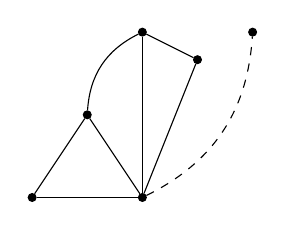
\begin{tikzpicture}[scale=0.7]
		\tikzset{vertex/.style = {shape=circle,draw, inner sep = 1pt, fill=black}}

		\node[vertex] (A_1) at (0,0) {};
		\node[vertex] (A_2) at (1,1.5) {};
		\node[vertex] (A_3) at (2,0) {};
		\node[vertex] (A_4) at (2,3) {};
		\node[vertex] (A_5) at (4,3) {};
		\node[vertex] (A_6) at (3,2.5) {};




		\draw (A_1)--(A_2);
		\draw (A_2)--(A_3);
		\draw (A_3)--(A_4);
		\draw (A_1)--(A_3);
		\draw (A_4)--(A_6);
		\draw (A_3)--(A_6);
		\draw[bend right, dashed] (A_3) to (A_5);
		\draw[bend left] (A_2) to (A_4);

	\end{tikzpicture}
	\hspace{40px}
	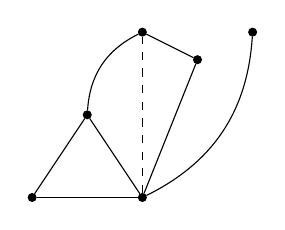
\begin{tikzpicture}[scale=0.7]
		\tikzset{vertex/.style = {shape=circle,draw, inner sep = 1pt, fill=black}}

		\node[vertex] (A_1) at (0,0) {};
		\node[vertex] (A_2) at (1,1.5) {};
		\node[vertex] (A_3) at (2,0) {};
		\node[vertex] (A_4) at (2,3) {};
		\node[vertex] (A_5) at (4,3) {};
		\node[vertex] (A_6) at (3,2.5) {};




		\draw (A_1)--(A_2);
		\draw (A_2)--(A_3);
		\draw[dashed] (A_3)--(A_4);
		\draw (A_1)--(A_3);
		\draw (A_4)--(A_6);
		\draw (A_3)--(A_6);
		\draw[bend right] (A_3) to (A_5);
		\draw[bend left] (A_2) to (A_4);

	\end{tikzpicture}
\end{center}

\begin{itemize}
	\item Jeśli po każdej ze stron rozpatrywanej krawędzi była inna ściana, to po usunięciu krawędzi dwie ściany scalą się w jedną.
	\item Gdy zaś po każdej ze stron tej krawędzi była ta sama ściana, to oznacza, że jej usunięcie rozspójni składową, do której ona należy, na dwie części.
\end{itemize}

\noindent
W pierwszym przypadku $f$ maleje o 1, a w drugim $c$ rośnie o $1$. W obu przypadkach z założenia indukcyjnego wyniknie teza.

\qed

\noindent
W powyższym rozumowaniu pominięto szczegóły formalne, zachęcamy uważną czytelniczkę/czytelnika, aby spróbował zrozumieć dokładnie, dlaczego powyższe rozumowanie jest poprawne.

\vspace{5px}

% Teraz dwa przykłady


% Przykład z pajączkami
% source:
\heading{Przykład 2}

\noindent
Dany jest graf o $n$ wierzchołkach posiadający $k$ krawędzi o numerach
będących różnymi liczbami całkowitymi od $1$ do $k$. Udowodnić, że istnieje w
nim ścieżka składająca się z co najmniej $\frac{2k}{n}$ krawędzi, których numery tworzą ciąg rosnący.

\vspace{5px}

\heading{Rozwiązanie}

\vspace{5px}
\noindent
Na każdym wierzchołku połóżmy kamień. Najpierw zamieńmy miejscami kamienie, które leżą na wierzchołkach krawędzi o numerze $1$, następnie te, które leżą na wierzchołkach krawędzi o numerze $2$, ..., aż zamienimy te, które leżą na wierzchołkach krawędzi o numerze $k$.

\vspace{10px}
\noindent
W każdym ruchu przesuwamy dwa kamienie. Więc łącznie wykonamy $2k$ przesunięć kamieni. Skoro kamieni jest $n$, to istnieje kamień przesunięty co najmniej $\frac{2k}{n}$~razy. Numery kolejnych rozpatrywanych krawędzi były coraz większe. Toteż ciąg krawędzi, przez które był on przekładany, jest poszukiwaną ścieżką. 

\qed

\noindent
Powyższe zadanie pokazuje, jak ważne jest próbowanie nietypowych pomysłów w matematyce. Nawet jeśli nie doprowadzą one bezpośrednio do rozwiązania zadania, tak jak w powyższym przypadku, to bardzo często wynikają z nich przydatne obserwacje.

\newpage